\chapter{Projeto}

(dar um nome melhor pra seção de solução escolhida)


\section{Esquema Elétrico}
Na área de atuadores, foi realizada uma análise do esquema elétrico fornecido pelo professor. A partir disso, verificaram-se as conexões da porta paralela, assim como os componentes e conexões utilizados. Abaixo estão as imagens do esquema original (Fig. \ref{fig:prof_schematic}) e do desenvolvido no KiCad (Fig. \ref{fig:kicad_schematic}).

\begin{figure}[H]
    \centering
    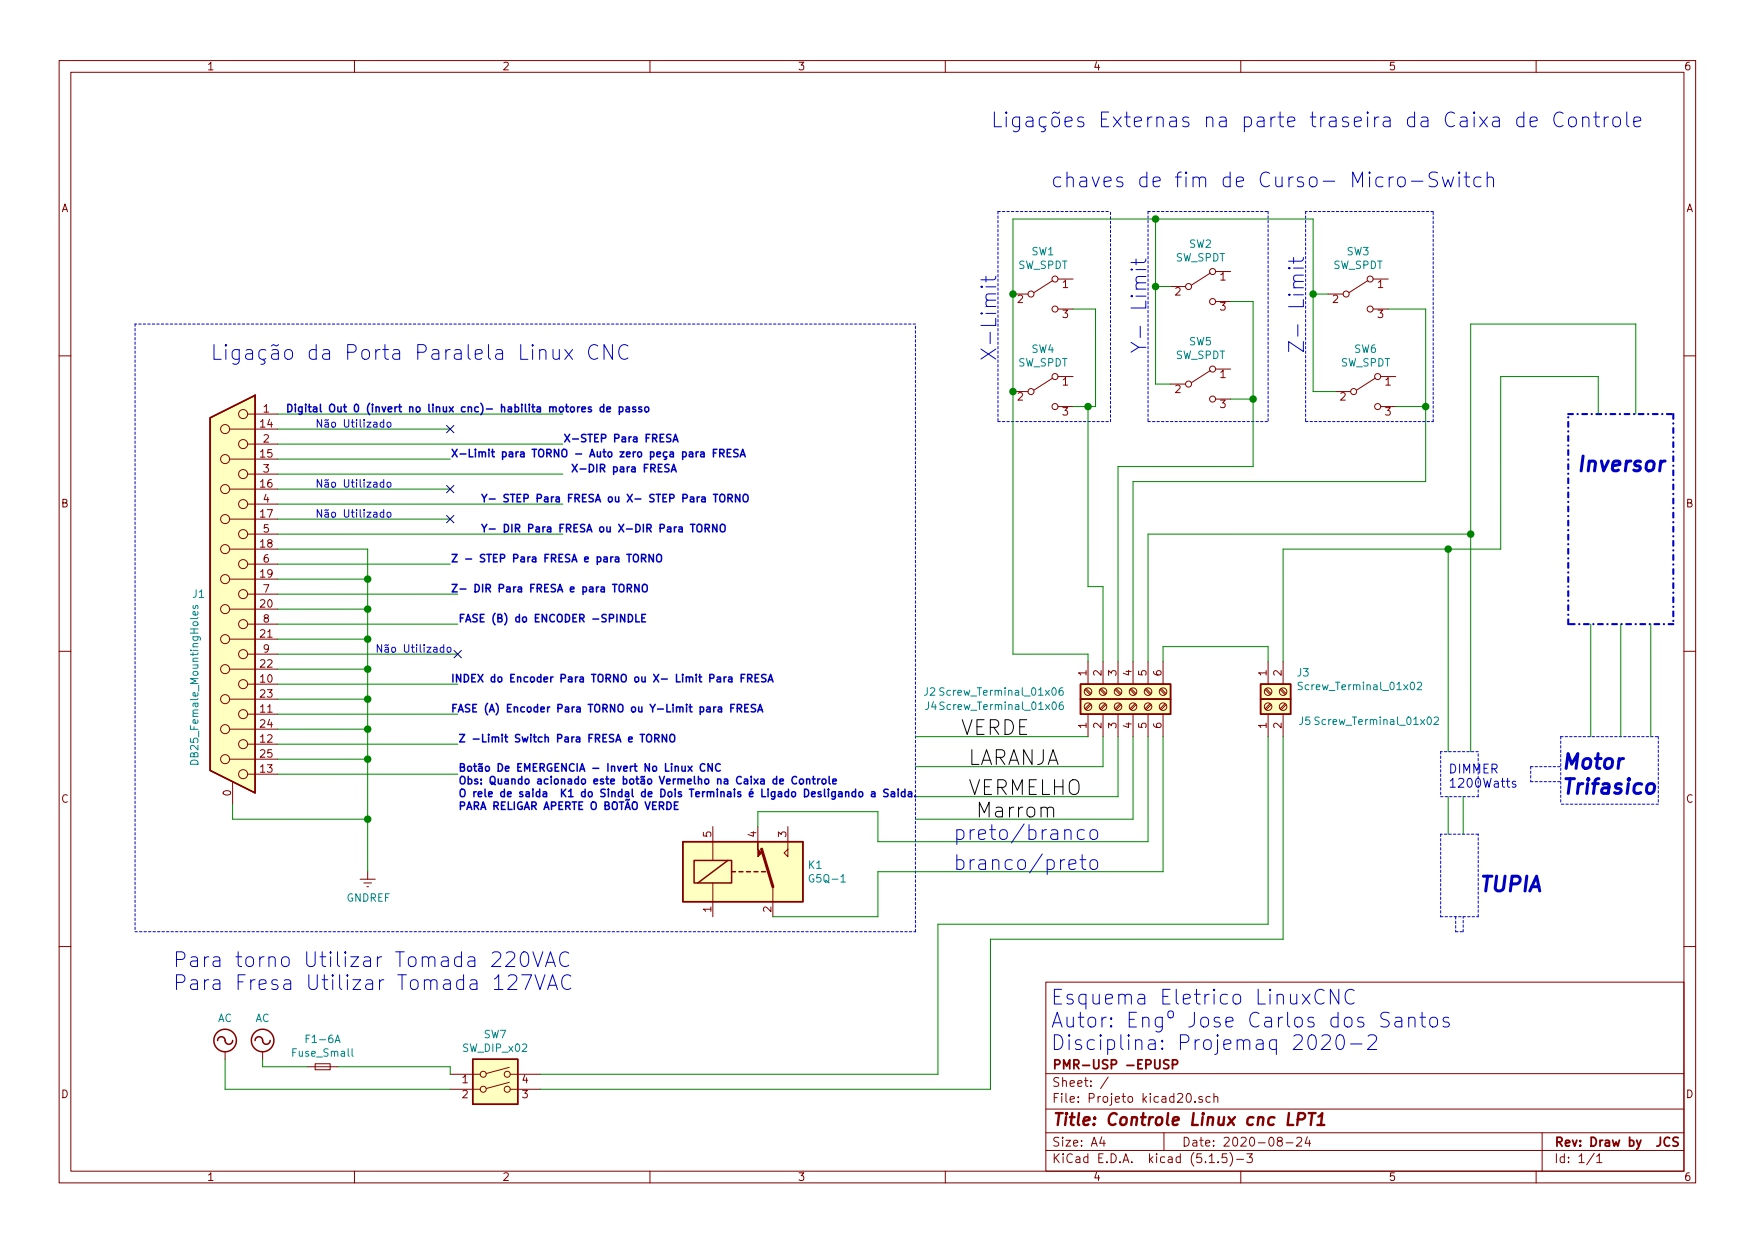
\includegraphics[width=\textwidth]{images/kicad-prof.jpg}
    \caption{Esquema elétrico fornecido pelo professor}
    \label{fig:prof_schematic}
\end{figure}

\begin{figure}[H]
    \centering
    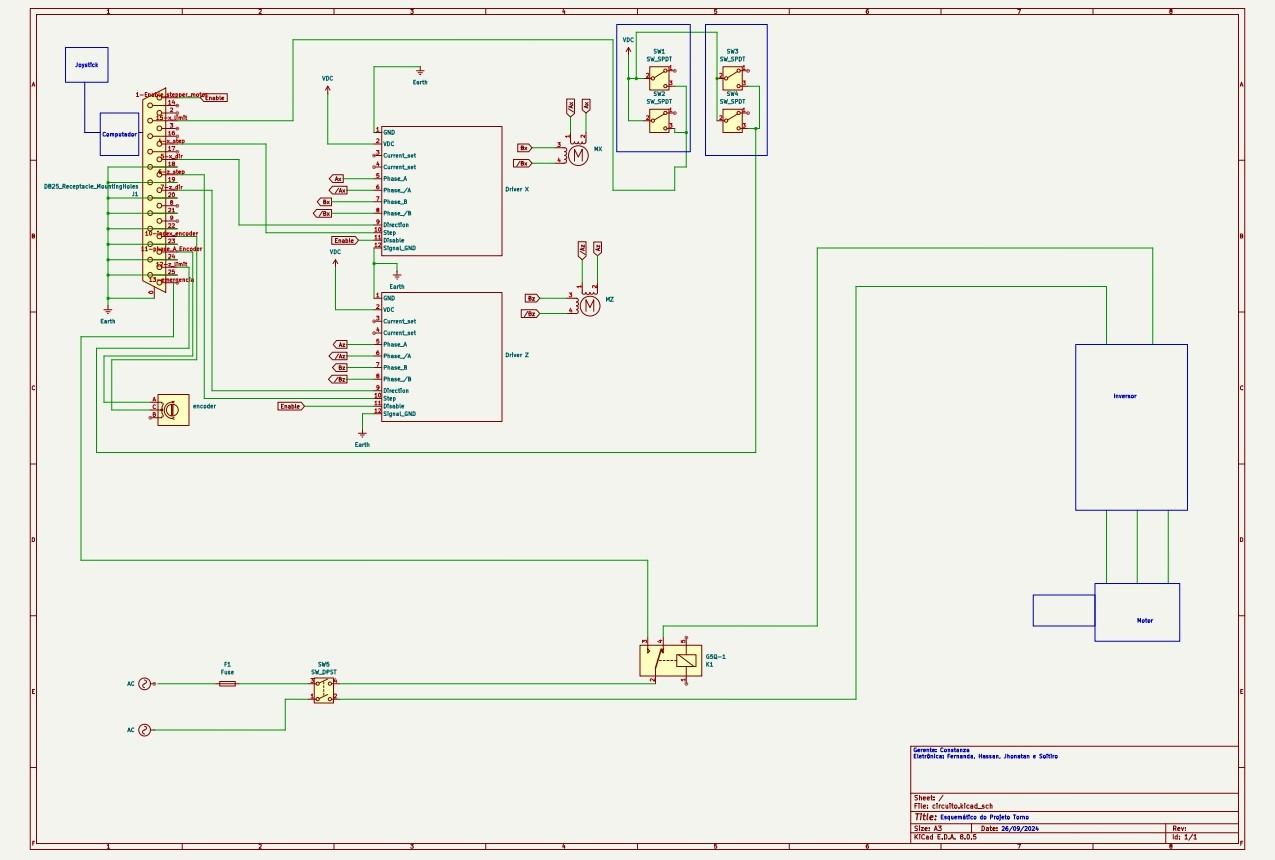
\includegraphics[width=\textwidth]{images/nosso-kicad.jpg}
    \caption{Esquema elétrico desenvolvido no KiCad}
    \label{fig:kicad_schematic}
\end{figure}

Algumas observações importantes incluem o fato de que o driver utilizado não estava disponível na biblioteca do KiCad, o que tornou necessário criá-lo seguindo as especificações técnicas de seu datasheet. No caso do encoder, foram consideradas apenas duas fases: a fase A e o index.

Para evitar "poluição visual", adotaram-se etiquetas para referenciar as conexões. Para o inversor e o motor, foi feito um esboço simplificado dos componentes, já que as suas características específicas não estavam presentes na biblioteca.


